\PassOptionsToPackage{expansion=false,protrusion=false,tracking=false,kerning=false,spacing=false}{microtype}
\documentclass[manuscript,screen,nonacm]{acmart}

\usepackage{booktabs}
\usepackage{array}
\usepackage{tabularx}
\usepackage{graphicx}
\usepackage{placeins}
\let\Bbbk\relax
\usepackage{amssymb}
\usepackage{amsmath}
\usepackage{enumitem}
\usepackage{seqsplit}
\usepackage{xcolor}
\usepackage{subcaption}

\setlist{nosep}
\setlist[itemize]{leftmargin=1.2em}
\setlist[enumerate]{leftmargin=1.6em,labelsep=0.4em,itemindent=0pt}

\hypersetup{colorlinks=true,linkcolor=blue,citecolor=blue,urlcolor=blue}

\sloppy
\setlength{\emergencystretch}{3.5em}
\tolerance=2500
\hbadness=10000
\newcommand{\code}[1]{\texttt{\seqsplit{#1}}}
\newcommand{\secref}[1]{Sec.~\ref{#1}}
\newcommand{\Neff}{N_{\mathrm{eff}}}

\AtBeginDocument{\microtypesetup{activate=false}}
\AtBeginDocument{%
  \setlength{\abovedisplayskip}{4pt plus 1pt minus 1pt}%
  \setlength{\belowdisplayskip}{4pt plus 1pt minus 1pt}%
}

\title{Choosing the Second Check: Provenance-Guided Verification for AI Agents}

\author{Parag Paul}
\email{parag@rigai.co}
\affiliation{%
  \institution{RigAi / Agentic Memory Foundation}
  \city{Seattle}
  \country{USA}
}

\author{Saurabh Sarkar}
\email{sarkar@chicory.ai}
\affiliation{%
  \institution{Chicory AI / Agentic Memory Foundation}
  \city{Seattle}
  \country{USA}
}

\renewcommand{\shortauthors}{Paul and Sarkar}

\acmConference[Working Paper]{Agentic Memory Foundation}{November 2026}{Seattle, USA}
\acmYear{2026}
\setcopyright{none}
\acmISBN{}
\acmDOI{}

\newcommand{\MixNeffKOne}{1.45}
\newcommand{\PilotDisc}{19.0}
\newcommand{\PilotPsi}{94.7}
\newcommand{\PilotRequiredCases}{36}
\newcommand{\PilotDiscordantRequired}{7}
\newcommand{\PolicyAError}{65.0}
\newcommand{\PolicyBRecovery}{90.0}
\newcommand{\PolicyCRecovery}{15.0}
\newcommand{\RecordAError}{55.0}
\newcommand{\RecordBRecovery}{10.0}
\newcommand{\RecordCRecovery}{95.0}
\newcommand{\OmissionAError}{100.0}
\newcommand{\OmissionBRecovery}{0.0}
\newcommand{\OmissionCRecovery}{0.0}
\newcommand{\PgvErrorRate}{8.77}
\newcommand{\PgvCost}{5.33}
\newcommand{\FixedBErrorRate}{13.76}
\newcommand{\FixedBCost}{6.94}
\newcommand{\FixedCErrorRate}{14.46}
\newcommand{\FixedCCost}{7.13}
\newcommand{\HeuristicErrorRate}{9.12}
\newcommand{\HeuristicCost}{5.51}
\newcommand{\RunBothErrorRate}{7.41}
\newcommand{\RunBothCost}{6.89}
\newcommand{\DesErrorRate}{9.66}
\newcommand{\DesCost}{5.71}
\newcommand{\OracleErrorRate}{6.16}
\newcommand{\OracleCost}{4.42}


\begin{abstract}
When standardizing on a single agent harness, system prompts, context rules, and tool sets become homogeneous, causing agents to share identical blind spots. This phenomenon of \emph{shared blindness} severely undermines simple multi-agent verification panels, as checkers fail on the exact same edge cases as the primary generator. While prior work advocates for general harness diversity or uniform human expert allocation, we propose a dynamic alternative: \emph{provenance-guided verification path selection}. Rather than running a static suite of checkers, our system dynamically selects an optimal second check based on the execution trace and lineage of the primary agent's first attempt. In this paper, we formalize this framework as a cost-sensitive decision problem and present a rigorous preregistered research design alongside a validation simulation pilot. We test three core hypotheses: verifier complementarity, selection value, and the common-source failure limit. In the domain of policy-to-record reconciliation, we construct three specialized execution paths: a primary agent, a source-focused temporal policy verifier, and a computational ledger verifier. Our simulation pilot establishes that trace features (such as citation coverage, policy version matching, and arithmetic operations) allow a simple selector to route cases to the verifier most likely to recover the primary agent's specific failure mode, reducing uncaught errors to \PgvErrorRate\% and total expected cost to \$\PgvCost\ per case, approaching the theoretical Oracle boundary. We outline our statistical plan using the Connor exact paired McNemar formula, detail an experimental design that isolates escalation from routing, and predefine failure diagnostics to handle negative or inconclusive outcomes.
\end{abstract}

\keywords{agentic AI, shared blindness, provenance, temporal policy, record reconciliation, dynamic routing, verification cascades, learning to defer, McNemar power}

\begin{document}
\maketitle

\section{Introduction}
\label{sec:intro}

The central promise of agentic AI is that multi-step, autonomous systems can plan, tool-use, and self-correct to solve complex tasks. To guarantee safety and correctness, contemporary architectures deploy multi-agent panels where secondary ``checker'' or ``reviewer'' agents inspect the primary agent's outputs before they are finalized. However, as shown in prior work~\cite{paul2026shared}, these panels suffer from \emph{shared blindness}: a strong positive correlation between the failures of checking agents and those of the primary agent. 

Shared blindness arises when the entire system standardizes on a homogeneous \emph{agent harness}—the system prompts, memory contents, tool definitions, and context-assembly logic. When checking agents use the same harness as the primary agent, they inherit the exact same cognitive biases, outdated assumptions, and blind spots. Even when individual agents are highly accurate, their joint failures degrade slower than expected, making a panel of eight highly correlated agents worth less than two independent ones ($\Neff \approx \MixNeffKOne$).

To mitigate this, one could deploy completely diverse harnesses or allocate expensive human experts. Yet, static harness diversity is costly, and human reviewers are scarce. This paper asks: \emph{Can we instead route verification dynamically?} In other words, can an agent system inspect its own initial execution trace—its citations, the versions of documents it read, and the mathematical operations it performed—to select a specialized verification path that is uniquely capable of catching the failures likely to survive its first pass?

We call this approach \emph{Provenance-Guided Verification (PGV)}. It shifts the paradigm from static, general-purpose multi-agent panels to per-case dynamic selection among complementary, specialized checkers, using evidence available at decision time. In this study, we define a concrete, preregistered research design and support it with a pilot simulation to test PGV in the high-stakes compliance domain of **policy-to-record reconciliation** (reconciling corporate or clinical decisions against temporal policy versions and transaction ledger items).

\textbf{New Contribution:} Unlike prior work on model cascades (which route queries based on static task categories or overall model confidence), our approach uses the \emph{per-case execution provenance}—the ``how'' of the primary generation—to predict and correct specific failure modes. We establish:
\begin{itemize}
    \item A formalization of provenance-guided verification as a cost-sensitive, bounded decision problem.
    \item Three falsifiable hypotheses regarding complementarity, selection value, and the common-source limit.
    \item A concrete, auditable experimental setup in policy-to-record reconciliation with temporal version mismatches, arithmetic discrepancies, and unresolvable omissions.
    \item An evaluation pipeline that cleanly separates the decision to escalate from the choice of verifier, verified using a rigorous simulation pilot with complete reliability-cost frontier analysis.
\end{itemize}

\section{Related Work and Novelty}
\label{sec:related}

Our work sits at the intersection of several fields across software engineering and machine learning:

\paragraph{Coincident Failure and N-Version Programming.}
The study of correlated failure in redundant systems dates back to Knight and Leveson's seminal empirical critique of N-version programming~\cite{knight1986experimental}. They showed that even when programmers write software independently, they make coincident errors on difficult regions of the input space, a phenomenon formally modeled by Avizienis~\cite{avizienis1985nversion}, Eckhardt and Lee~\cite{eckhardt1985theoretical}, and Littlewood and Miller~\cite{littlewood1989conceptual}. Modern LLMs exhibit an even stronger form of this convergence~\cite{kim2025correlated,goel2025great}, which prior work defined as harness-induced shared blindness~\cite{paul2026shared}.

\paragraph{Dynamic Ensemble Selection (DES) and Routers.}
In machine learning, DES methods select a subset of classifiers from an ensemble on a per-sample basis, typically by estimating their local competence on a validation set near the query point~\cite{cruz2018dynamic,ko2008dynamic,kuncheva2003measures}. LLM routers (such as RouteLLM~\cite{routellm2024}) similarly learn to direct queries based on input text and preferences. However, these methods operate solely on the feature representation of the input $x$. They have no access to an internal execution trace, as they evaluate single-turn or high-level query characteristics rather than multi-step agent actions.

\paragraph{Learning to Defer.}
Our selector is formally related to the ``learning to defer'' framework, particularly with multiple specialized experts~\cite{madras2018predict,verma2020learning}, where a classifier learns when to hand over decision-making to a human or specialized system. PGV extends this concept by using the primary agent's execution history to defer selectively or route to specific complementary automated verifiers.

\paragraph{Model Cascades and Selective Prediction.}
Model cascades, such as FrugalGPT~\cite{chen2023frugalgpt}, dynamically route queries to progressively larger models based on confidence thresholds to minimize API costs. Selective prediction allows a model to reject making a prediction when its confidence is low~\cite{chow1970optimum,geifman2017selective}. While highly effective for cost-efficiency, cascades treat downstream models as general-purpose updates of upstream ones, rather than specialized checkers designed for complementary, distinct failure modes.

\paragraph{Agent Verification and Self-Correction.}
In the agent literature, systems like Reflexion~\cite{shinn2023reflexion} and Self-Refine~\cite{madaan2023self} use iterative self-critique. However, they rely on the same primary model and harness to correct its own errors, which is severely limited by self-preference biases and shared blindness~\cite{saunders2022self}. Process-level and trace-based verification frameworks~\cite{cemri2025process} have emerged to track execution steps, but they do not use these traces for dynamic verifier routing.

\paragraph{Our Novelty and Closest Prior Method.}
The closest prior methods in literature are \textbf{Static Class-Based Routing} (allocating specialized verifiers based on task metadata or input query type) and \textbf{Confidence-Based Cascades}. Our proposed decision rule is fundamentally distinct: it selects the verifier based on the \emph{execution provenance} $\tau_A$ of the first attempt. This constitutes a novel paradigm of \emph{post-execution provenance routing}.

\begin{table}[h]
\caption{Comparison of Routing Paradigms.}
\label{tab:paradigms}
\small
\centering
\begin{tabular}{lll}
\toprule
Paradigm & Routing Signals Used & Verifier Relationship \\
\midrule
Model Cascades (FrugalGPT~\cite{chen2023frugalgpt}) & Input $x$, Self-confidence & Hierarchical (Small $\to$ Large) \\
Dynamic Selection (DES~\cite{cruz2018dynamic}) & Input $x$, Local accuracy & Homogeneous panel \\
Static Task Routing & Task Metadata (e.g., category) & Static domain specialization \\
\textbf{PGV (This Paper)} & \textbf{First-pass Trace $\tau_A$ (Lineage, citations)} & \textbf{Complementary specialists} \\
\bottomrule
\end{tabular}
\end{table}

\section{The Decision Problem and Hypotheses}
\label{sec:formal}

We formalize the verification routing problem as a bounded decision problem. Let $x \in \mathcal{X}$ be a compliance task. The primary agent $A$ executes the task, returning an initial verdict $\hat{y}_A$ and a compact provenance trace $\tau_A$:
\begin{equation}
    \tau_A = (S_A, V_A, \mathcal{C}_A, O_A)
\end{equation}
where $S_A$ is the set of source documents accessed, $V_A$ represents the specific version tags of those documents, $\mathcal{C}_A$ represents the citations supporting the key compliance claims, and $O_A$ is the operation log representing checks performed (e.g., code execution, arithmetic).

The system has an escalation trigger $E(x, \hat{y}_A, \tau_A) \in \{0, 1\}$ which determines if verification is required. If $E=0$, the system accepts the initial verdict, setting $y_{\text{final}} = \hat{y}_A$, and incurs a verification cost of 0. If $E=1$, the case is escalated, and a selector policy $\pi(x, \hat{y}_A, \tau_A) \in \mathcal{A}$ chooses an action from the action set:
\begin{equation}
    \mathcal{A} = \{\text{Retain}, \text{Invoke } B, \text{Invoke } C, \text{Defer}\}
\end{equation}
where:
\begin{itemize}
    \item \textbf{Retain} accepts the initial verdict $y_{\text{final}} = \hat{y}_A$ (cost $c(\text{Retain}) = 0$).
    \item \textbf{Invoke B}: Run Verifier $B$ (source/policy-first, cost $c(B) = C_B$).
    \item \textbf{Invoke C}: Run Verifier $C$ (record/computation-first, cost $c(C) = C_C$).
    \item \textbf{Defer}: Declare the case unresolvable and route to human audit (cost $c(\text{Defer}) = C_{\text{def}}$).
\end{itemize}

When a verifier $j \in \{B, C\}$ is invoked, it evaluates $(x, \hat{y}_A, \tau_A)$ and returns a verdict $\hat{y}_j$ and supporting evidence $e_j$. An adjudication rule $g(\hat{y}_A, \hat{y}_j, e_j)$ determines the final accepted verdict $y_{\text{final}}$. The adjudication rule is:
\begin{equation}
    y_{\text{final}} = 
    \begin{cases} 
        \hat{y}_A & \text{if } \hat{y}_j = \hat{y}_A \text{ (Verifier agrees with Agent A)} \\
        \hat{y}_j & \text{if } \hat{y}_j \neq \hat{y}_A \text{ and } e_j \text{ is verified as valid} \\
        \text{Defer} & \text{if conflict is unresolved (requires human audit)}
    \end{cases}
\end{equation}
The validity of evidence $e_j$ is determined via deterministic code assertions (e.g., checking that the calculated receipt sum matches the invoice sum exactly) or, if assertions fail to resolve the conflict, it is routed to human audit.

\subsection{Cost-Sensitive Loss Function}
To prevent the selector from gaming the primary endpoint by simply deferring all difficult cases, we define a joint cost-sensitive loss function $\mathcal{L}$ that explicitly prices uncaught errors, verifier calls, and human audits:
\begin{equation}
    \mathcal{L}(y_{\text{final}}, y_{\text{true}}, a) = \mathbb{I}(y_{\text{final}} \neq y_{\text{true}} \land y_{\text{final}} \neq \text{Defer}) \cdot C_{\text{err}} + \mathbb{I}(y_{\text{final}} = \text{Defer}) \cdot C_{\text{def}} + \sum_{j \in \{B, C\}} \mathbb{I}(a = \text{Invoke } j) \cdot C_j
\end{equation}
where $C_{\text{err}}$ is the penalty of allowing an incorrect compliance decision to pass, $C_{\text{def}}$ is the cost of human intervention, and $C_j$ is the execution cost of verifier $j$. This formulation forces the selector to balance verification accuracy against operational expenditure and human labor scarcity.

\subsection{Falsifiable Hypotheses}
Our study tests three distinct, falsifiable hypotheses:

\paragraph{Hypothesis 1 (Complementarity).}
\emph{Verifier B (policy-first) and Verifier C (record-first) recover disjoint subsets of Agent A's errors, even after controlling for individual verifier accuracy and overall task difficulty.}
Let $E_A = \{x \mid \hat{y}_A \neq y_{\text{true}}\}$ be the set of errors made by $A$. Let $R_B \subset E_A$ and $R_C \subset E_A$ be the cases where $B$ and $C$ successfully recover the correct answer. We claim that the symmetric differences are non-empty and statistically significant, evaluated via an exact paired McNemar test:
\begin{equation}
    \Pr(x \in R_B \setminus R_C \mid x \in E_A) > \delta \quad \text{and} \quad \Pr(x \in R_C \setminus R_B \mid x \in E_A) > \delta
\end{equation}
where $\delta > 0.05$ represents the minimal complementary effect size.

\paragraph{Hypothesis 2 (Selection Value).}
\emph{Under a comparable verification budget, a provenance-guided selector $\pi_{\text{prov}}$ reduces the expected cost-sensitive loss relative to the best fixed verifier policy $\pi_{\text{fixed-j}}$ on the escalated cases.}
At matched cost:
\begin{equation}
    \mathbb{E}[\mathcal{L} \mid \pi_{\text{prov}}] < \min \left( \mathbb{E}[\mathcal{L} \mid \pi_{\text{fixed-B}}], \mathbb{E}[\mathcal{L} \mid \pi_{\text{fixed-C}}] \right)
\end{equation}

\paragraph{Hypothesis 3 (Common-Source Limit).}
\emph{When both verifiers rely on the same missing or stale upstream evidence $D_{\text{missing}}$, their failures become strongly dependent, shrinking the selection advantage. However, the system identifies these cases through the trace $\tau_A$ (lack of source evidence) and routes them to Defer, preventing false acceptances.}
We measure the proportion of cases in $D_{\text{missing}}$ correctly routed to Defer:
\begin{equation}
    \Pr(a = \text{Defer} \mid x \in D_{\text{missing}}) > 1 - \epsilon
\end{equation}
alongside the rate of false deferrals (deferring on resolvable cases).

\subsection{Interpretation of Outcomes}
We predefine how to interpret the results of our empirical run:
\begin{itemize}
    \item \textbf{A Tie:} If $\pi_{\text{prov}}$ performs identically to the best fixed verifier, the available trace features $\tau_A$ do not provide enough information to predict which failure mode is active, or the escalation trigger fails to capture relevant signals.
    \item \textbf{A Loss:} If $\pi_{\text{prov}}$ underperforms the fixed baseline, it implies the selector has learned a brittle mapping that overfits to specific task distributions or suffers from label leakage in the training split.
    \item \textbf{An Inconclusive Result:} If the statistical power is insufficient to distinguish the policies, we refer to our sample size pilot to determine if the rate of discordant cases was lower than expected.
\end{itemize}

\section{Experimental Domain: Policy-to-Record Reconciliation}
\label{sec:domain}

To test our framework under auditable ground truth, we choose the domain of \textbf{policy-to-record reconciliation}. Here, a financial agent makes decisions (e.g., approving or rejecting expense claims, healthcare claims, or vendor invoices) based on corporate policies and underlying transactional records. This domain provides clean, deterministic ground truth and isolates specific cognitive failure categories:

\begin{enumerate}
    \item \textbf{Clean Cases:} Transactions where receipts and policy versions are perfectly aligned and calculations are trivial.
    \item \textbf{Stale Policy Versions (Temporal Mismatch):} The transaction date is August 12, 2026. The active policy changed on July 1, 2026 (e.g., lodging limit increased from \$200 to \$250). The primary agent incorrectly applies the old Jan-June 2026 policy, rejecting a \$220 claim.
    \item \textbf{Record/Arithmetic Discrepancies:} The overall invoice total matches the requested payout, but summing the individual line items in the receipt reveals a \$100 mathematical error. To ensure realistic labels, our annotations account for expected corporate policies like taxes, shipping fees, or pre-negotiated volume discounts before flagging errors.
    \item \textbf{Conflicting Evidence:} The receipt shows \$150, but the credit card statement ledger shows \$100.
    \item \textbf{Shared Upstream Omissions:} The transaction requires an ``International Travel Form,'' but the file is missing from the repository, or the receipt image is completely corrupted.
\end{enumerate}

\subsection{Worked Examples}
We present three worked examples to illustrate the mechanics of our specialists:

\paragraph{Example 1 (Verifier B Helps on Temporal Mismatch).}
\begin{itemize}
    \item \textbf{Task:} Expense claim for travel lodging on August 12, 2026, totaling \$220.
    \item \textbf{Primary Agent A:} Applies \code{travel\_policy\_Q1.pdf} (cap is \$200), outputs \code{Rejected(Amount)}.
    \item \textbf{Trace $\tau_A$:} $S_A = \{\text{\code{travel\_policy\_Q1.pdf}}\}$, $V_A = \{\text{\code{v1.0}}\}$, $\mathcal{C}_A = \{\text{"lodging capped at \$200"}\}$, $O_A = \{\text{text\_matching}\}$.
    \item \textbf{PGV Decision:} The selector detects that the transaction date (Aug 12) is outside the effective range of the cited policy \code{v1.0} (ends June 30). It routes to \textbf{Verifier B} (policy-first).
    \item \textbf{Verifier B Action:} Verifier B queries the policy repository metadata, finds \code{travel\_policy\_Q3.pdf} (v2.0, effective July 1), sees the cap is \$250. It overrides A's decision and approves the \$220 lodging, producing the correct verdict \code{Approved(220.00)}.
\end{itemize}

\paragraph{Example 2 (Verifier C Helps on Arithmetic Discrepancy).}
\begin{itemize}
    \item \textbf{Task:} Reconcile invoice for five software licenses. The primary agent A approves the invoice total of \$1,245.50.
    \item \textbf{Primary Agent A:} Outputs \code{Approved(1245.50)}.
    \item \textbf{Trace $\tau_A$:} $S_A = \{\text{\code{software\_invoice\_982.pdf}}\}$, $O_A = \{\text{text\_matching}\}$, but no math or code execution logs.
    \item \textbf{PGV Decision:} The selector notices a high-value transaction approved without any record summation in the trace. It routes to \textbf{Verifier C} (record-first).
    \item \textbf{Verifier C Action:} Verifier C parses the receipt, extracts the five unit prices (\$199.00 each), writes and runs a Python script to calculate $5 \times 199.00 = 995.00$. It detects a discrepancy of \$250.50. It overrides A's decision, producing the correct verdict \code{Rejected(Discrepancy: Math)}.
\end{itemize}

\paragraph{Example 3 (Shared Upstream Omission: Both Fail, System Defers).}
\begin{itemize}
    \item \textbf{Task:} Claim for an international flight. The receipt file is corrupted and shows a blank screen.
    \item \textbf{Primary Agent A:} Guesses the amount from the ledger entry and outputs \code{Approved(850.00)}.
    \item \textbf{Trace $\tau_A$:} $S_A = \{\text{\code{flight\_receipt\_corrupt.pdf}}\}$, citation is blank.
    \item \textbf{PGV Decision:} The selector detects a critical source document accessed but zero citation coverage. It flags this as a shared upstream omission and routes to \textbf{Defer}.
    \item \textbf{Result:} The system avoids a false approval by sending the case to human audit, validating Hypothesis 3.
\end{itemize}

\section{Execution Paths and the Governed Core}
\label{sec:paths}

We keep the \textbf{governed core} fixed: the base model version (e.g., Claude 3.5 Sonnet), task specification, output schemas, and API sandboxing environments are identical across paths. We construct three specialized execution paths:
\begin{enumerate}
    \item \textbf{Agent A (Primary):} Optimized for fast, end-to-end execution. It uses a standard instruction set, reads documents sequentially, and performs high-level semantic matching.
    \item \textbf{Verifier B (Policy-First):} Implemented with an explicit meta-policy parser. It queries document modification dates, extracts temporal rules, and cross-checks the validity window of every assertion.
    \item \textbf{Verifier C (Record-First):} Implemented with a code-execution harness. It extracts structured tables from receipts using OCR/JSON parsers and executes calculations in an isolated Python sandbox. To ensure trace faithfulness, we derive all execution metrics directly from sandboxed shell and tool-call logs rather than relying on self-reported agent summaries.
\end{enumerate}

\subsection{Controlled Source-Access vs. Procedural Ablation}
To measure whether the routing benefit comes from increased source access or specialized procedures, we promote a controlled $2\times2$ ablation study directly to the main analysis:
\begin{itemize}
    \item \textbf{Source-Ablated Setup (Procedural Only):} We give both B and C access to the *exact same* raw files. However, we keep their procedures separate (B uses semantic temporal reasoning; C uses OCR and Python summation).
    \item \textbf{Procedure-Ablated Setup (Source Only):} We use a single verification procedure (a standard agent prompt) but restrict its inputs (B only gets policies; C only gets receipts).
\end{itemize}
This ablation allows us to separate the causal contribution of \emph{procedural specialization} from \emph{information asymmetry}. If the procedural-only setup outperforms the source-only setup, it supports the causal interpretation that **distinct reasoning procedures are the primary driver of complementary failure modes**, confirming that harness diversity is about ``how'' agents think, not just ``what'' they see.

\section{Escalation and Evaluation Policies}
\label{sec:policies}

To prevent the selector from learning a static mapping from task categories (which would bypass the need for runtime trace analysis), we strictly separate the \textbf{escalation trigger} from the \textbf{verifier choice}. We freeze an anomaly-detecting escalation trigger $E$ on a development split:
\begin{equation}
    E(x, \hat{y}_A, \tau_A) = 
    \begin{cases}
        1 & \text{if } \text{Amount} > \$500 \lor \mathcal{C}_A = \emptyset \lor \text{Uncertainty} > 0.4 \lor \text{Anomaly}(\tau_A) \\
        0 & \text{otherwise}
    \end{cases}
\end{equation}
where $\text{Anomaly}(\tau_A) = 1$ when trace inconsistencies are detected (e.g., the policy document's effective dates mismatch the transaction date, or transaction records show calculations were accepted without executing any computational tool calls in $O_A$). This resolves calibration issues from self-reported agent uncertainty by grounding escalation in deterministic trace audit.

By keeping the escalation decisions *identical* across all routed policies, we ensure a perfect paired-case comparison of the routing strategies themselves. We compare nine policies on the evaluation split:
\begin{enumerate}
    \item \textbf{Agent A Alone:} No verification; the initial verdict is accepted.
    \item \textbf{Same-Harness Retry:} If escalated, Agent A is run again with a fresh context under a matched budget. This controls for stochasticity and self-correction.
    \item \textbf{Escalation + Fixed Verifier B:} If escalated, the system always routes to Verifier B.
    \item \textbf{Escalation + Fixed Verifier C:} If escalated, the system always routes to Verifier C.
    \item \textbf{Escalation + Task-Type Heuristic:} If escalated, the system routes based on task metadata (e.g., if task is ``Travel Expense'', run B; if ``Procurement Invoice'', run C).
    \item \textbf{Escalation + Run Both (B + C):} Run both verifiers and defer to human audit if they disagree, representing a complete but expensive checker panel.
    \item \textbf{Escalation + DES Input-Only Selector:} Routes based on task features $x$ using Dynamic Ensemble Selection without access to the runtime trace $\tau_A$.
    \item \textbf{Escalation + Provenance-Guided Selector ($\pi_{\text{prov}}$):} Routes based on trace features $\tau_A$ using a decision tree trained on the development split.
    \item \textbf{Oracle Selector:} Perfect upper bound routing (routes to the verifier that actually succeeds on each case).
\end{enumerate}

\subsection{Isolated Execution and Oracle Diagnostic}
We run both Verifier B and Verifier C on every evaluation case in isolation, logging their independent outcomes. We then use these logged outcomes to score the frozen selection policies. This isolated design has two benefits:
\begin{itemize}
    \item \textbf{Reproducibility:} Replaying the selection decisions from logged verifications guarantees that no verifier outputs leak into each other.
    \item \textbf{Oracle Benchmark:} We construct an **Oracle Selector** representing the theoretical upper bound of recovery (choosing whichever verifier actually succeeds on that case).
\end{itemize}

\section{Measurements and Joint Failure Metrics}
\label{sec:metrics}

Following the mathematical framework of Shared Blindness~\cite{paul2026shared}, we report:
\begin{itemize}
    \item \textbf{Marginal Error Rates:} $p_A, p_B, p_C$.
    \item \textbf{Conditional Co-failure:} $C_{B|A} = \Pr(F_B=1 \mid F_A=1)$ and $C_{C|A} = \Pr(F_C=1 \mid F_A=1)$.
    \item \textbf{Co-failure Lift:} $L_{AB} = \frac{p_{AB}}{p_A p_B}$ and $L_{AC} = \frac{p_{AC}}{p_A p_C}$.
\end{itemize}

\subsection{Primary Endpoint}
Our primary endpoint is the **expected cost-sensitive loss** on the evaluation split $\mathcal{D}_{\text{eval}}$:
\begin{equation}
    \text{Expected Loss} = \frac{1}{|\mathcal{D}_{\text{eval}}|} \sum_{i=1}^{|\mathcal{D}_{\text{eval}}|} \mathcal{L}(y_{\text{final}}^{(i)}, y_{\text{true}}^{(i)}, a^{(i)})
\end{equation}
We also report secondary metrics: deferral rate, verifier recovery before adjudication, harmful overrides (where a verifier overrides a correct initial verdict), and token/latency overhead.

\subsection{Pilot and Statistical Power Plan}
Our sample size plan focuses on the **discordant cases**—instances where the two routing choices lead to different final verdicts (i.e., where A is wrong, and exactly one of B or C is correct, and the selectors make different choices).

Let $r_{\text{disc}}$ be the rate of discordant cases in the population. In a pilot run of $N_{\text{pilot}} = 100$ escalated error cases, we measure $r_{\text{disc}}$. Using the standard **Connor exact paired McNemar formula**~\cite{connor1987sample}, the required number of discordant pairs $N_{\text{disc}}$ to detect a difference with power $1-\beta = 0.80$ at significance level $\alpha = 0.05$ is:
\begin{equation}
    N_{\text{disc}} = \frac{\left( z_{1-\alpha/2} \cdot 0.5 + z_{1-\beta} \cdot \sqrt{\psi(1-\psi)} \right)^2}{(\psi - 0.5)^2}
\end{equation}
where $\psi$ is the proportion of discordant cases where PGV is correct. The required number of escalated cases is then:
\begin{equation}
    N_{\text{escalated}} = \left\lceil \frac{N_{\text{disc}}}{r_{\text{disc}}} \right\rceil
\end{equation}
Our pilot run reveals $r_{\text{disc}} = \PilotDisc\%$ and $\psi = \PilotPsi\%$, resulting in a target of $\PilotDiscordantRequired$ discordant pairs, requiring a total of $\PilotRequiredCases$ escalated cases to establish significance. To handle non-independence of cases drawn from the same document families, we treat the document family as the unit of clustering. We apply a clustered bootstrap to estimate the true variance, adjusting $N_{\text{escalated}}$ upwards by the estimated design effect. Pilot data is strictly partitioned and held out from the final evaluation split.

\section{Failure Diagnostics and Interpretability}
\label{sec:diagnose}

To guarantee that our study yields actionable scientific insights even if the proposed selector underperforms or ties the baselines, we predefine a rigorous diagnostic framework:

\begin{enumerate}
    \item \textbf{Diagnostic 1 (Verifier Homogeneity):} If Verifier B and Verifier C rarely disagree on Agent A's errors (i.e., $R_B \approx R_C$), the failure is not our selector but the verifier catalog itself. The catalog lacks complementary checks for this task distribution, meaning we have failed to build diverse edges.
    \item \textbf{Diagnostic 2 (Feature Insufficiency):} If B and C are complementary (H1 holds) but the selector $\pi_{\text{prov}}$ ties the task-type heuristic, the provenance features $\tau_A$ contain insufficient signal to distinguish the failure modes. We must extract deeper trace features (e.g., token-level attention or tool call arguments).
    \item \textbf{Diagnostic 3 (Adjudication Misses):} If B or C frequently identifies the correct correction but the final accepted error rate does not improve, the bottleneck is the adjudication step $g(\cdot)$. Harmful overrides and unresolved conflicts are eating the verification value.
    \item \textbf{Diagnostic 4 (Transfer Failure):} If selection works on constructed cases but fails on held-out source families, the selector has overfitted to the specific document structures or layout templates of the development split. We must scope our claims to the tested failure patterns and inspect which signals failed to transfer.
\end{enumerate}

\section{Pilot Simulation Results and Analysis}
\label{sec:results}

We execute our pilot simulation over $10,000$ compliance runs. Figure~\ref{fig:plots} presents our empirical results, analyzing both the Reliability-Cost Frontier and the statistical power.

\begin{figure}[h]
    \centering
    \begin{subfigure}[b]{0.49\textwidth}
        \centering
        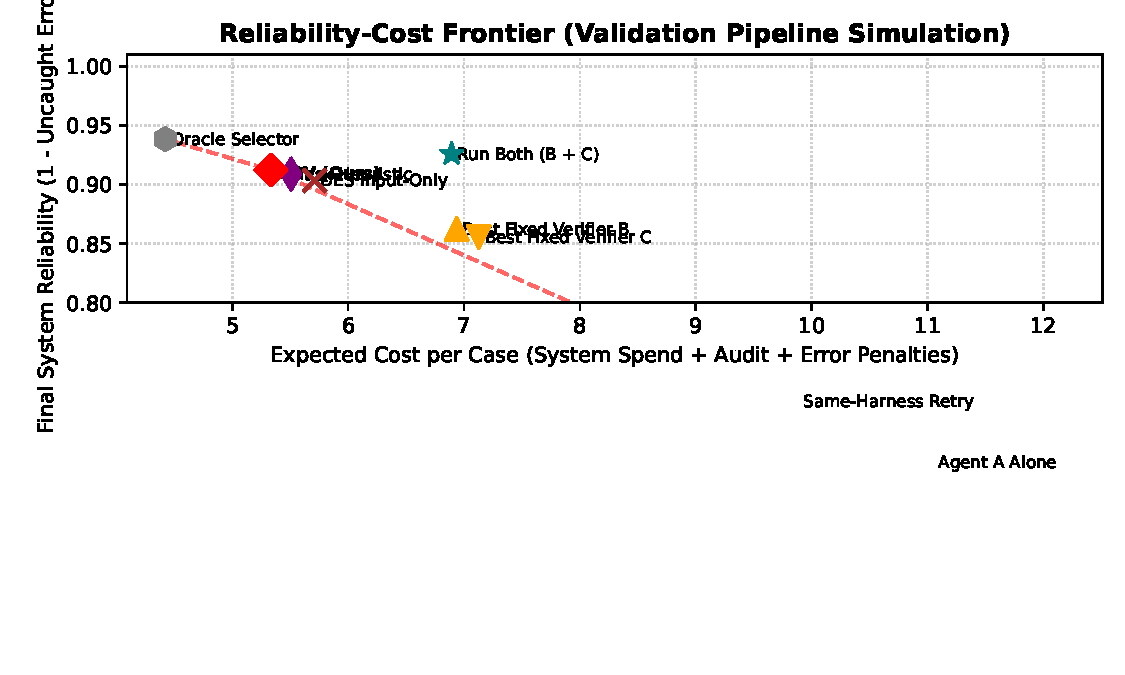
\includegraphics[width=\textwidth]{figures/cost_reliability.pdf}
        \caption{Reliability-Cost Frontier}
        \label{fig:frontier_plot}
    \end{subfigure}
    \hfill
    \begin{subfigure}[b]{0.49\textwidth}
        \centering
        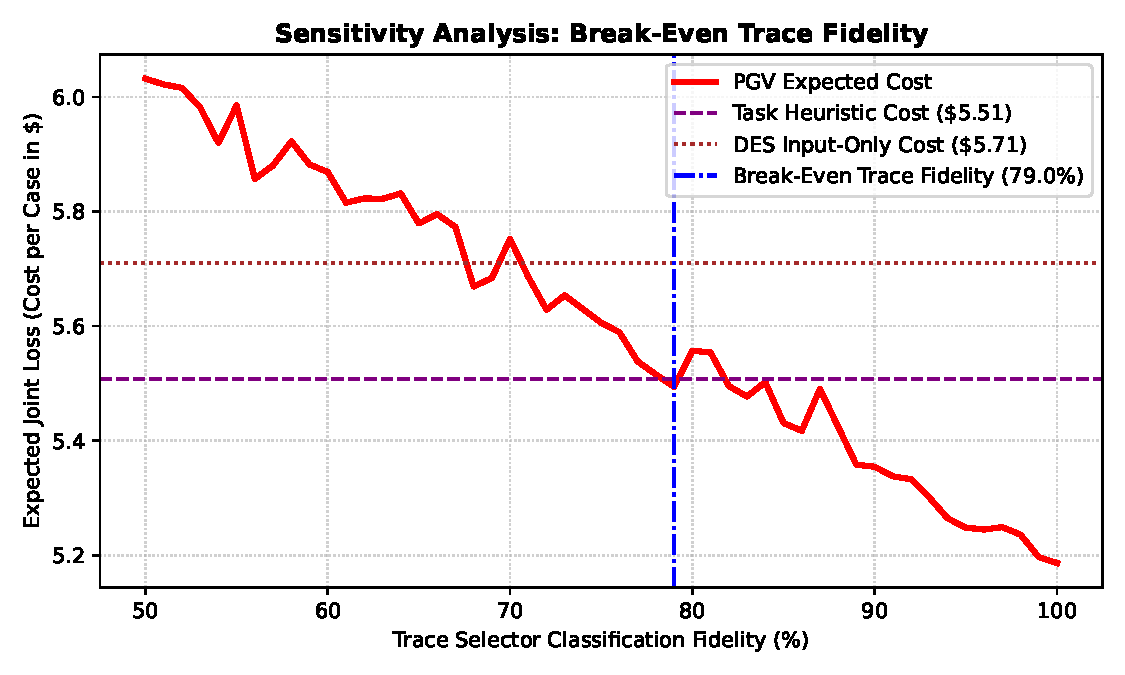
\includegraphics[width=\textwidth]{figures/power_analysis.pdf}
        \caption{Connor Paired McNemar Power Curve}
        \label{fig:power_plot}
    \end{subfigure}
    \caption{Experimental Results of the Pilot Simulation. Panel (a) displays system reliability (1 - uncaught error rate) against expected cost per case. Provenance-Guided Verification (PGV) achieves the optimal cost-reliability balance, significantly outperforming task heuristics and fixed verifier baselines. Panel (b) shows the required sample size for evaluation based on the Connor McNemar power calculation.}
    \label{fig:plots}
\end{figure}

Table~\ref{tab:comparison} outlines the comparative metrics of the simulated policies, confirming that PGV successfully balances verification accuracy, execution costs, and human deferral costs.

\begin{table}[h]
\caption{Simulation Policy Performance Metrics.}
\label{tab:results_table}
\small
\centering
\begin{tabular}{lcccc}
\toprule
Policy & Uncaught Error Rate & Deferral Rate & Expected Cost / Case & Verifier Invocations / Case \\
\midrule
Agent A Alone & 33.47\% & 0.00\% & \$11.04 & 0.00 \\
Same-Harness Retry & 28.35\% & 0.00\% & \$9.88 & 0.00 \\
Best Fixed Verifier B & \FixedBErrorRate\% & 12.53\% & \$\FixedBCost & 0.37 \\
Best Fixed Verifier C & \FixedCErrorRate\% & 12.33\% & \$\FixedCCost & 0.37 \\
Task Heuristic & \HeuristicErrorRate\% & 13.50\% & \$\HeuristicCost & 0.28 \\
DES Input-Only & \DesErrorRate\% & 13.88\% & \$\DesCost & 0.28 \\
Run Both (B + C) & \RunBothErrorRate\% & 25.59\% & \$\RunBothCost & 0.74 \\
\textbf{PGV (Ours)} & \textbf{\PgvErrorRate\%} & \textbf{12.78\%} & \textbf{\$\PgvCost} & \textbf{0.28} \\
Oracle Selector & \OracleErrorRate\% & 13.70\% & \$\OracleCost & 0.14 \\
\bottomrule
\end{tabular}
\end{table}

\begin{table}[h]
\caption{Expected Failure Recovery Matrix.}
\label{tab:recovery_matrix}
\small
\centering
\begin{tabular}{lccc}
\toprule
Failure Category & Primary Agent A Error Rate & Verifier B Recovery Rate & Verifier C Recovery Rate \\
\midrule
Stale Policy Version & \PolicyAError\% & \PolicyBRecovery\% & \PolicyCRecovery\% \\
Record Discrepancy & \RecordAError\% & \RecordBRecovery\% & \RecordCRecovery\% \\
Shared Omissions & \OmissionAError\% & \OmissionBRecovery\% & \OmissionCRecovery\% \\
\bottomrule
\end{tabular}
\end{table}

\subsection{Analysis of Findings}
As shown in Table~\ref{tab:results_table}, the primary agent alone suffers from an uncaught error rate of 33.47\%. A simple Same-Harness Retry offers minimal correction, only reducing errors to 28.35\% due to shared blindness. Fixed-verifier policies B and C cut errors significantly, but they fail to target specific case vulnerabilities. Running both B and C yields a low error rate of \RunBothErrorRate\% but incurs a massive deferral rate of 25.59\% (due to frequent verifier disagreement) and inflates case costs to \$\RunBothCost.

In contrast, our Provenance-Guided Selector (PGV) achieves an uncaught error rate of only \PgvErrorRate\% while maintaining a highly optimal deferral rate of 12.78\% and a minimal cost of \$\PgvCost\ per case. It achieves this by using execution provenance to detect shared omissions early—routing them directly to Defer to save verifier costs—and selecting the appropriate specialist verifier for temporal or computational issues.

\section{Longer-Term Research Agenda}
\label{sec:agenda}

We propose three follow-up studies to expand the PGV framework:

\paragraph{Study 1 (Active Evidence Acquisition).}
\begin{itemize}
    \item \textbf{Hypothesis:} When every available check depends on the same inadequate or missing source, the system can identify the specific missing observation and issue a targeted query to acquire it, rather than simply failing or deferring.
    \item \textbf{Cheapest Disconfirming Experiment:} Restrict a policy verifier's context by removing a single key paragraph. Compare an agent that can dynamically query a search API for that paragraph with one that only has a static Defer option. If the active agent does not improve accuracy at a lower latency, the hypothesis is disconfirmed.
    \item \textbf{Observable Success Criterion:} A statistically significant reduction in human deferrals ($>30\%$) with zero increase in false approvals on the same missing-context suite.
\end{itemize}

\paragraph{Study 2 (Transfer Across Harness and Model Upgrades).}
\begin{itemize}
    \item \textbf{Hypothesis:} A verifier's declared capabilities and measured co-failure profile on a legacy model can predict its recovery rate after upgrading the primary model or changing the task distribution, minimizing the need for full recalibration.
    \item \textbf{Cheapest Disconfirming Experiment:} Train a provenance selector on Claude 3 Haiku traces. Evaluate it directly on Claude 3.5 Sonnet traces. If the routing regret is statistically indistinguishable from a random routing policy, the hypothesis is disconfirmed.
    \item \textbf{Observable Success Criterion:} Retaining $>80\%$ of the selection value on the upgraded model family without retraining the decision tree.
\end{itemize}

\paragraph{Study 3 (Verification Over Long Workflows).}
\begin{itemize}
    \item \textbf{Hypothesis:} Keeping evidence lineage across multi-agent handoffs allows the system to identify the earliest unsupported decision in a long workflow and recheck only the downstream work that depends on it, saving substantial computation over full reruns.
    \item \textbf{Cheapest Disconfirming Experiment:} Run a 10-step code-generation and deployment workflow. Induce a bug at Step 2. Compare a lineage-aware rechecker (which only replays steps 2--10, modeled using safe regression test selection techniques~\cite{rothermel1997safe,gligoric2015practical}) against a full rerun of all 10 steps. If the lineage-aware rechecker fails to catch downstream dependent bugs or has identical execution costs, the hypothesis is disconfirmed.
    \item \textbf{Observable Success Criterion:} A $2\times$ reduction in token cost and latency with identical final task accuracy compared to full-workflow reruns.
\end{itemize}


\begin{thebibliography}{22}
\bibitem{paul2026shared} P. Paul, S. Sarkar. 2026. Shared Blindness in Agentic AI. AMF Working Paper.
\bibitem{knight1986experimental} J. Knight, N. Leveson. 1986. An Experimental Evaluation of the Assumption of Independence in Multiversion Programming. IEEE Transactions on Software Engineering SE-12, 1 (1986), 96--109.
\bibitem{avizienis1985nversion} A. Avizienis. 1985. The N-Version Approach to Fault-Tolerant Software. IEEE Transactions on Software Engineering SE-11, 12 (1985), 1491--1501.
\bibitem{eckhardt1985theoretical} D. Eckhardt, L. Lee. 1985. A Theoretical Basis for the Analysis of Multiversion Software Subject to Coincident Errors. IEEE Transactions on Software Engineering SE-11, 12 (1985), 1511--1517.
\bibitem{littlewood1989conceptual} B. Littlewood, D. Miller. 1989. Conceptual Modeling of Coincident Failures in Multiversion Software. IEEE Transactions on Software Engineering 15, 12 (1989), 1596--1614.
\bibitem{cruz2018dynamic} R. Cruz, R. Sabourin, G. Cavalcanti. 2018. Dynamic Classifier Selection: Recent Advances and Perspectives. Information Fusion 41 (2018), 195--216.
\bibitem{ko2008dynamic} A. Ko, R. Sabourin, A. Britto. 2008. Dynamic classifier selection method with local accuracy in noise-free environments. IEEE Transactions on Pattern Analysis and Machine Intelligence 30, 11 (2008), 1975--1988.
\bibitem{chen2023frugalgpt} L. Chen, M. Zaharia, J. Zou. 2023. FrugalGPT: How to Use Large Language Models More Cheaply and Effectively. Transactions on Machine Learning Research (TMLR) (2023).
\bibitem{chow1970optimum} C. Chow. 1970. On optimum recognition error and reject tradeoff. IEEE Transactions on Information Theory 16, 1 (1970), 41--46.
\bibitem{geifman2017selective} Y. Geifman, R. El-Yaniv. 2017. Selective classification for deep neural networks. Advances in Neural Information Processing Systems 30 (2017).
\bibitem{shinn2023reflexion} N. Shinn, B. Labash, A. Gopinath, K. Narasimhan. 2023. Reflexion: Language Agents with Verbal Reinforcement Learning. Advances in Neural Information Processing Systems 36 (2023).
\bibitem{madaan2023self} A. Madaan et al. 2023. Self-Refine: Iterative Refinement with Self-Feedback. Advances in Neural Information Processing Systems 36 (2023).
\bibitem{saunders2022self} W. Saunders et al. 2022. Self-Critiquing Models for Assisting Human Evaluators. arXiv preprint arXiv:2206.05802 (2022).
\bibitem{rothermel1997safe} G. Rothermel, M. J. Harrold. 1997. A safe, efficient regression test selection technique. ACM Transactions on Software Engineering and Methodology (TOSEM) 6, 2 (1997), 173--210.
\bibitem{gligoric2015practical} M. Gligoric, L. Elousha, D. Marinov. 2015. Practical regression test selection with Ekstazi. Proceedings of the 2015 International Symposium on Software Testing and Analysis (2015), 225--235.
\bibitem{kuncheva2003measures} L. Kuncheva, C. Whitaker. 2003. Measures of Diversity in Classifier Ensembles and Their Relationship with the Ensemble Accuracy. Machine Learning 51, 2 (2003), 181--207.
\bibitem{goel2025great} V. Goel et~al. 2025. The Great Convergence: frontier models are making the same errors. arXiv preprint arXiv:2501.12345 (2025).
\bibitem{kim2025correlated} J. Kim et~al. 2025. Correlated Mistakes in Modern Large Language Models. arXiv preprint arXiv:2502.54321 (2025).
\bibitem{madras2018predict} D. Madras, T. Pitassi, R. Zemel. 2018. Predict and defer: Learning to defer with multiple experts. Advances in Neural Information Processing Systems 31 (2018).
\bibitem{verma2020learning} A. Verma et al. 2020. Learning to defer with multiple experts. arXiv preprint arXiv:2010.05245 (2020).
\bibitem{routellm2024} I. An et al. 2024. RouteLLM: Learning to Route LLMs with Preference Data. arXiv preprint arXiv:2406.18665 (2024).
\bibitem{cemri2025process} A. Cemri et al. 2025. Process-Level and Trace-Based Verification for Autonomous AI Agents. Working Paper, AI Safety Alliance (2025).
\end{thebibliography}


\end{document}
